\textbf{Nagerune}\\
Denne rune siges at være den ældste rune, der eksisterer. Dens kræfter bruges med offensivt henblik. Dette var også den første rune, som thanen Even Ûhr Krezz opdagede, da han fandt runernes kraft dybt i sit folks bjerge.\\
\begin{figure}[H]
    \centering
    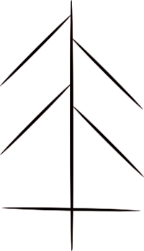
\includegraphics[height=5.5cm]{setup/Pictures/Nagerune.png}
    \caption{Nagerune}
\end{figure}

\textbf{Elementrune}\\
Denne rune besidder alle elementernes kræfter. Hvordan den er opstået ved ingen præcist, men dværgene har dog legender, der fortæller om et uhyre, som levede i fortiden som skabte denne rune. Elementrunens kræfter kan være både offensive og defensive.\\
\begin{figure}[H]
    \centering
    
\includegraphics[height=5.5cm]{setup/Pictures/Elementrune.png}
    \caption{Elementrune}
\end{figure}

\textbf{Jernrune}\\
Denne rune er skabt til beskyttelse. Ifølge legenden blev den skabt af thanen Altika, som levede generationen efter Even Ûhr Krezz. Til tider er denne rune også kendt for at have
helbredende egenskaber.
\begin{figure}[H]
    \centering
    
\includegraphics[height=5.5cm]{setup/Pictures/Jernrune.png}
    \caption{Jernrune}
\end{figure}

\textbf{Dragerune}\\
Den nyeste rune, som først lige er blevet magtfuld. Med ophøjelsen af Esselia og dragernes Opvågning, har denne rune nu fået ny magt, som forstyrrer balancen.\\
\begin{figure}[H]
    \centering
    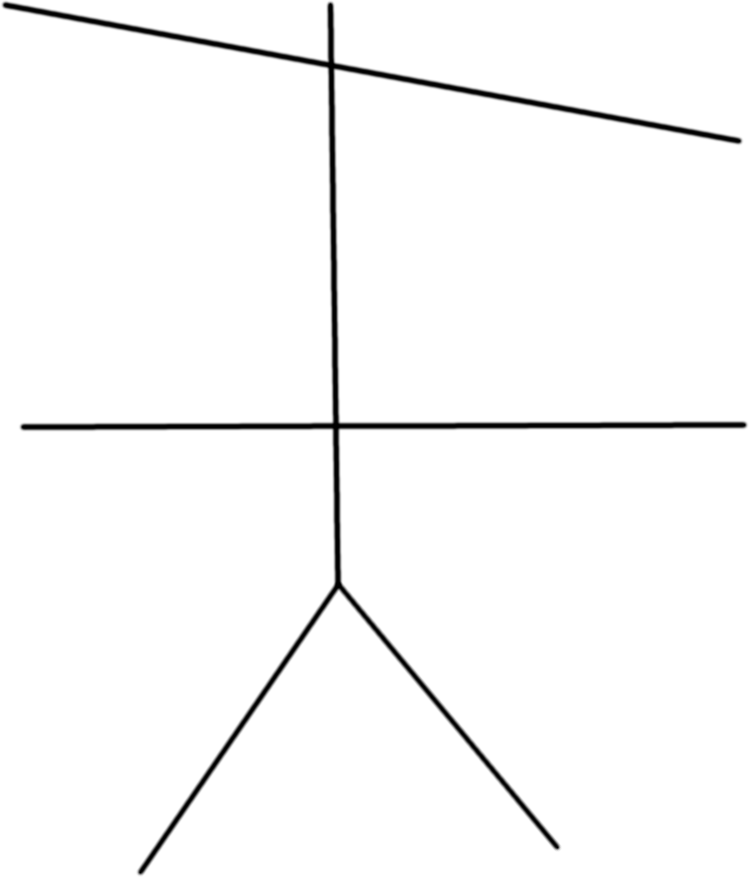
\includegraphics[height=5.5cm]{setup/Pictures/Dragerune.png}
    \caption{Dragerune}
\end{figure}

\begin{runeskjold*}[Drageskind]
\textbf{Effekt:} Du tager kun halvt så meget skade fra magier. (rundet op)\\
\textbf{Ingredienser:} 3 Elementruner, 3 Drageruner, 2 Jernruner.
\end{runeskjold*}

\begin{runeskjold*}[Essalias beskyttelse]
\textbf{Effekt:} Du får dobbelt så meget liv når du bliver helbredt.\\
\textbf{Ingredienser:} : 1 Elementrune, 1 Dragerune.
\end{runeskjold*}

\begin{runeskjold*}[Krigerens Skjold]
\textbf{Effekt:} Dette skjold giver dig 1 RP på samme måde som en normal rustningsdel vil. Det ekstra RP fra dit skjold vil altid være det første du mister; dette ekstra RP mistes kun når du selv rammes og ikke når nogen slår på skjoldet. Dette RP kan repareres som normalt hos en smed.\\
\textbf{Ingredienser:} : 1 Jernrune.
\end{runeskjold*}

\begin{runeskjold*}[Magiens Bane]
\textbf{Effekt:} Dette runeskjold gør bæreren i stand til 2 gange per døgn, at modstå en valgfri magi som rammer spilleren. Når spilleren rammes af en magi, de vil beskyttes imod, skal de udtale kommandoen: ”Magiens Bane – immun!”\\
\textbf{Ingredienser:} 4 Jern, 2 Jernruner, 2 Elementruner, 1 Dragerune.
\end{runeskjold*}

\begin{runevåben*}[Armens styrke]
\textbf{Effekt:} Bæreren af dette våben vil modtage 5 ekstra NK så længe de har våbenet på sig.\\
\textbf{Ingredienser:} 1 Nagerune
\end{runevåben*}

\begin{runevåben*}[Heksejægeren]
\textbf{Effekt:} En gang per døgn kan du ophæve en magi, hvis du rammer en person eller barriere med dette våben. Du kan ikke ophæve magiske genstande, såsom talismaner med dette våben.\\
\textbf{Ingredienser:} 1 Jern, 1 Sjælestøv, 1 Nagerune, 1 Jernrune, 1 Elementrune, 1 Dragerune.
\end{runevåben*}

\begin{runevåben*}[Kellwans Klinge]
\textbf{Effekt:} Dette våben giver permanent hellig skade. Dette skal som normalt markeres med et grønt bånd. (For optimal effekt kan dette også siges ved slag på fjender, hvor hellig skade kan have effekt.)\\
\textbf{Ingredienser:} 1 Nagerrune, 1 Elementrune.
\end{runevåben*}

\begin{runevåben*}[Livets Le]
\textbf{Effekt:} Når du dræber en person med dette våben vil du genvinde 1 mistet LP. Du kan ikke gå over din maksimale LP ved brug af dette våben.\\
\textbf{Ingredienser:} 1 Flagermuse gødning, 1 Elementrune, 2 Nagerruner, 1 Dragerune
\end{runevåben*}

\begin{runevåben*}[Magerens Mareridt]
Dette våben har ingen effekt i kamp. Det kan bruges til tortur, hvor den vil syge vilje og fokus fra ethvert offer. Tortureres en person med mana i kroppen, vil de miste mana i stedet for LP, med samme interval på 1 mana per minut. Offerets mana kan først genvindes 1 time efter torturen er afsluttet. Har offeret ingen mana (tilbage) i kroppen, vil de miste LP som ved normal tortur.
Note: Denne rune genstand tæller ikke mod det samlet antal rune genstande du må have på dig. Denne rune kan sættes på alle torturinstrumenter.\\
\textbf{Ingredienser:} 1 Nagerrune, 1 Enhjørningeblod.
\end{runevåben*}

\begin{runerustning*}[Dragens Rustning]
\textbf{Effekt:} 2 gange pr. scenarie kan du ved at berøre nogen bruge kommandoen: ”Drageild – 6 hellig skade”. Du vælger selv hvornår du bruger kommandoen.\\
\textbf{Ingredienser:} 4 Sulfur, 2 Dragerune, 2 Elementrune, 1 Ildgræs.
\end{runerustning*}

\begin{runerustning*}[Gudernes Rustning]
\textbf{Effekt:} Negative magier påvirker dig nu kun halvt så lang tid (rundet op.)\\
\textbf{Ingredienser:} 3 Drageruner, 1 Elementrune.
\end{runerustning*}

\begin{runerustning*}[Hærførens Rustning]
\textbf{Effekt:} Denne rustning giver dig 3 ekstra RP. Disse RP fungerer på samme måde som de normale RP du får fra en normal rustning. De ekstra RP vil altid være det første, du mister og de sidste der, bliver repareret.\\
\textbf{Ingredienser:} 4 Jern, 3 Jernruner.
\end{runerustning*}

\begin{runerustning*}[Jordens Rustning]
\textbf{Effekt:} Du bliver immun overfor alle vælte effekter\\
\textbf{Ingredienser:} 2 Jernruner, 2 Elementruner, 1 Flagermuse gødning.
\end{runerustning*}

\begin{runerustning*}[Krigerens Rustning]
\textbf{Effekt:} Denne rustning giver dig 2 ekstra RP. Disse RP fungerer på samme måde som de normale RP du får fra en normal rustning. De ekstra RP vil altid være det første, du mister og de sidste der, bliver repareret.\\
\textbf{Ingredienser:} 2 jern, 1 Jernrune.
\end{runerustning*}

\begin{runerustning*}[Samaritanernes Rustning]
\textbf{Effekt:} Hvis du går på 0 LP mens du bærer denne rustning, vil du automatisk genvinde alle dine naturlige LP 10 minutter efter du vågner; dvs. når du igen er kampdygtig ifølge dødsreglerne, som findes i det almindelige regelsæt.\\
\textbf{Ingredienser:} 1 Jernrune, 1 Enhjørningeblod.
\end{runerustning*}

\begin{runerustning*}[Thanens Rustning]
\textbf{Effekt:} Denne rustning reparerer alt din udrustning på mystisk vis. Dette betyder, at du genvinder 1 RP pr. 2. minut når du bærer rustningen og er ved bevidsthed. Du kan ikke genvinde mere RP end du normalt får for din rustning.\\
\textbf{Ingredienser:} 1 Jernrune, 1 Elementrune.
\end{runerustning*}